\pdfminorversion=4
\documentclass{beamer}
%\usetheme[compress]{Berlin}

\usepackage[utf8]{inputenc}
\usepackage[english]{babel}
\usepackage{default}
\usepackage{graphicx}
\usepackage{amsmath}
\usepackage{overpic}
\usepackage{geometry}
\usepackage{subfigure}
\usepackage{calc}
\usepackage{comment}
\usepackage{bigints}
\usepackage{multimedia}

\renewcommand{\thesubfigure}{}
\setbeamertemplate{navigation symbols}{}
%\setbeamertemplate{headline}{}
\setbeamertemplate{footline}{}

\usepackage{tikz}
\usetikzlibrary{calc}

\tikzset{egrid/.style={draw,help lines}}
\tikzset{mgrid/.style={draw,help lines,dashed}}
\tikzset{epoint/.style={draw,circle,red,inner sep=2pt,fill}}
\tikzset{mpoint/.style={draw,circle,blue,inner sep=2pt,fill}}

\usetheme{Frankfurt}

\newcommand{\odvod}[2]{\frac{\partial #1}{\partial #2}}
\renewcommand{\vec}{\mathbf}
\newcommand{\eps}{\varepsilon}
\newcommand{\E}{\vec E}
\newcommand{\B}{\vec B}
\newcommand{\angl}[1]{(\textit{angl. #1})}
\newcommand{\ticssize}{\fontsize{9}{10}\selectfont}
\newcommand{\backupbegin}{
   \newcounter{finalframe}
   \setcounter{finalframe}{\value{framenumber}}
}
\newcommand{\backupend}{
   \setcounter{framenumber}{\value{finalframe}}
}

\newcommand{\stalno}[2]{
  \begin{overpic}[width=.23\textwidth,trim=-1cm -1cm -1cm -1cm]{./Defekti/g_defect_#2}\end{overpic} 
  \begin{overpic}[width=.23\textwidth]{./Slike/lic_#1_1}\put(2,88){\color{white} \large \bf 1 $\boldsymbol\mu$m}\end{overpic} 
  \begin{overpic}[width=.23\textwidth]{./Slike/lic_#1_37}\put(2,88){\color{white} \large \bf 10 $\boldsymbol\mu$m}\end{overpic} 	
  \begin{overpic}[width=.23\textwidth]{./Slike/lic_#1_50}\put(2,88){\color{white} \large \bf 15 $\boldsymbol\mu$m}\end{overpic}
}

\newenvironment{slide}[1]{\subsection{#1}\begin{frame}\frametitle{#1}}{\end{frame}}

\graphicspath{ {./Slike/}{./Video/} }

\begin{document}
\title[ILCC 2018]{Optical properties of heliconical liquid crystals}
\author[Anja Bregar]{\begin{tabular}{rl} \underline{Anja Bregar}, Mitja Štimulak and Miha Ravnik \end{tabular}}
\institute[FMF]{Faculty of Mathematics and Physics, University of Ljubljana}

\date{\today}

\section{Introduction}

\begin{slide}{}
 \titlepage
\end{slide}


\begin{slide}{Motivation}
   \begin{itemize}
  \item $\vec{n}=(\cos \varphi(z)  \sin \theta, \sin \varphi (z) \sin \theta, \cos \theta), \, \mathrm{where } \,\, \varphi(z) = 2 \pi z/ p \,\, \mathrm{and} \,\, \theta=\mathrm{const.} $
   \begin{center}
    \begin{overpic}[height=90pt]{./figures/helikoniki-skica2} 
%     %\put(10,-10) {\tiny Rybin et al., Nat. Commun. (2015)}
    \end{overpic}
    \begin{overpic}[height=90pt]{./figures/refraction-ellipsoid}
%     %\put(10,-10) {\tiny Rybin et al., Nat. Commun. (2015)}
    \end{overpic}
   \end{center}
    \item Early experiments: X-ray range, pitch $\sim 10 \mathrm{nm}$ (bent-core LC)
   \begin{center}
    \begin{overpic}[height=50pt]{./figures/tunable-small-pitch-clark}
    \put(10,-6) {\tiny FFTEM images, $p\approx 14 \, \mathrm{nm}$. }
    \put(5,-12) {\tiny Chen et al., PRE 89, 022506 (2014). }
    %\put(10,-10) {\tiny Chen, Nakata, Shao, Tuchband, Shuai, Baumeister, Weissflog, Walba, Glaser, Maclennan, Clark, PRE 89, 022506 (2014). }
   \end{overpic}
   \end{center}
   \vspace{0.3cm}
   \item Optical range: LC of rod-like units linked by a flexible chain
    \begin{center}
    \begin{overpic}[height=55pt]{./figures/lavrentovich-advMat-2015}
    %\put(10,-2) {\tiny J. Xiang, Y. Li, Q. Li, D. A. Paterson, J. M. D. Storey, C. T. Imrie and O. D. Lavrentovich, Adv. Mater. 27, 3014 (2015). }
    \end{overpic}
    
    \vspace{-0.1cm}
    {\tiny Xiang et al., Adv. Mater. 27, 3014 (2015). }
    \end{center}
    \end{itemize}
% %     \begin{exampleblock}{}
% %     $\lambda \approx a$: diffraction\\
% %     $\lambda \approx 3a$: photonic crystal\\
% %     $\lambda \approx 10a$: metamaterial
% %    \end{exampleblock}
   \vspace{-0.5cm}

\end{slide}


\begin{slide}{Experimental examples}
   \vspace{-0.3cm}
   \fontsize{10}{10}
   \begin{itemize}
   \item Arises for LC with $K_3 \ll K_2$ for a range of $\vec{E}_{ext}$
   \begin{center}
     \begin{overpic}[height=60pt]{./figures/electrooptic-response-helicoid}
    %\put(12,-3) {\tiny Xiang, Shiyanovskii, Imrie, Lavrentovich, PRL 112, 217801 (2014). }
      \put(12,-3) {\tiny Xiang et al., PRL 112, 217801 (2014). }
     \end{overpic}
  \end{center}    
    \item Possibility of shifting $p$ and $\theta$ with external electric field $\vec{E_{ext}}$
    \item Theoretical dependence of $p$ and $\theta$ vs. $\vec{E_{ext}}$
    \vspace{-0.1cm}
    {\tiny J. Xiang, S. V. Shiyanovskii, C. Imrie and O. D. Lavrentovich, Phys. Rev. Lett. 112, 217801 (2014). }
%     \begin{overpic}[height=55pt]{./figures/electric-field-dependence-theoretical}
%     \put(10,-2) {\tiny J. Xiang, S. V. Shiyanovskii, C. Imrie and O. D. Lavrentovich, Phys. Rev. Lett. 112, 217801 (2014). }
%    \end{overpic}
   \end{itemize}
%  \begin{columns}[c]
%   \column{.4\textwidth}
%    \center
% %    \begin{overpic}[height=80pt]{./slike/resonant-mtm1}
% %    \end{overpic}
% %    \begin{overpic}[height=80pt]{./slike/resonant-mtm2}
% %     \put(-60,-10) {\tiny L. Zhang et. al., Phys. Rev. B (2013)}
% %    \end{overpic}
%   \column{.55\textwidth}
% %    \begin{overpic}[height=80pt]{./slike/neg-refractive-index2}
% %     \put(10,-10) {\tiny C. M. Soukoulis, M. Wegener, Nat. Photon. (2011)}
% %    \end{overpic}
%  \end{columns}
\end{slide}



\begin{slide}{Contents}
 \begin{itemize}
  \item Shifting of heliconical band gap with changing material properties
  \item Electric $\vec{E}$ and magnetic $\vec{H}$ fields inside heliconics -- eigenmodes
  \item Winding of the Poynting vector $\vec{P}$ 
  \item Outlook
  \end{itemize}
\end{slide}



\section{Band gap shifting}

\begin{slide}{Methods}
  \begin{itemize}
    \item FDTD
    \item MPB
  \end{itemize}
\end{slide}

\begin{slide}{Analysis of $\vec{E}$ and $\vec{D}$ fields}
\begin{columns}[c]
  \begin{column}{.78\textwidth}
    \begin{itemize}
      \item On-axis propagation: $\vec{D} \perp \vec{k}$ $\rightarrow$ $\vec{D}$ stays in plane of boundary 
      \item Since $D_z=0$ for heliconics, we can follow the derivation of the band-gap for cholesterics
      \item Light of same handedness as structure: has band gap, opposite handednesses: no band gap
    \item Effective periodicity: $p/2$
    \end{itemize}
  \end{column}
  \begin{column}{.22\textwidth}
    \centering
    \begin{overpic}[height=84pt]{./figures/twoLayer-refraction-sketch}
    \end{overpic}
    \begin{overpic}[height=75pt]{./figures/refraction-ellipsoid}
    \end{overpic}   
  \end{column}
\end{columns}
\end{slide}



\begin{slide}{Opening of the BG with $\theta$}
  \vspace{-0.5cm}
  \fontsize{10}{10}
  \begin{itemize}
    \item BG boundaries depend on $n_o$ and effective extraordinary refractive index $n_e^{eff}=\dfrac{n_o*n_e}{\sqrt{n_o^2 \sin^2 \theta + n_e^2 \cos^2 \theta}}$
    \item BG for vacuum wavelengths between 
    \vspace {-0.3cm}
    \begin{align*}
      p \, n_o < \lambda_0 < p \, n_e^{eff} \, &, \quad n_o < n_e \\
      p \, n_o > \lambda_0 > p \, n_e^{eff} \, &, \quad n_e < n_o 
      \label{eq:bg}
    \end{align*}
  \end{itemize}
  \centering
  \begin{overpic}[height=110pt]{./figures/band-gap-theta}
  \end{overpic}  
\end{slide}



\begin{slide}{Transmittivity}
\begin{itemize}
  \item Band gap width depends on $\theta$
  \item Central position of band gap depends on $p$
    \begin{overpic}[height=90pt]{./figures/transmittivity-heliconics}
    \end{overpic}
\item From transmittivity spectra $\rightarrow$ $p$ and $\theta$ determined uniquely
\item Connection between $E_{ext}$ and $p$ and $\theta$: Xiang et al., PRL 112, 217801 (2014)
\end{itemize}
\end{slide}




\section{Eigenmodes of $\vec{E}$}

\begin{slide}{Band gap edge modes}
\fontsize{10}{10}
\begin{itemize}
    \item $\vec{E} \nparallel \vec{D}$ since $\vec{D} = \varepsilon_0 \underline{\underline{\varepsilon}} \vec{E}$
    \item In cholesterics: $E_z = 0$, in heliconics: $E_z \neq 0$
    \item On band gap edge: Eigenmodes right- or left-circularly polarized waves with additional $E_z$-component
\end{itemize}
\vspace{0.3cm}
      \centering
      \begin{overpic}[height=130pt]{./figures/Ebands-near-BG-v2.pdf}
      \end{overpic}  
\end{slide}



\begin{slide}{Dependence of $E_z$ on $\lambda$}
\fontsize{10}{10}
\begin{itemize}
  \item $E_z$ oscillates sinusoidally: $E_z$ will be the same in size when $xy$-angle between $\vec{D}$ and $\vec{n}$ increases by $2 m \pi$, $m \in \mathbb{Z}$.  
  \item $\lambda_z^{LCP} = \dfrac{\lambda p}{p+\lambda}, \quad \lambda_z^{RCP} = \pm \dfrac{\lambda p}{p-\lambda}$, always $\lambda_z^{RCP}>\lambda_z^{LCP}$
  \item RCP: $E_z$ constant, $\lambda_z \rightarrow \infty$ when on edge of BG, otherwise it is smaller and depends on $\lambda/p$
  \item LCP: $\lambda_z = \lambda/2$ on edge of BG
\end{itemize}
\centering
  \begin{overpic}[height=95pt]{./figures/Ez-dependence}
  \end{overpic}
\end{slide}


\begin{slide}{Poynting vector}
\vspace{-0.7cm}
\begin{itemize}
  \item if $E_z \neq 0 \rightarrow P_{xy} \neq 0$
  \item Poynting vector rotates about the propagation axis
  \item<1> RCP: wavelength of $E_z$ rotation increases when nearing the band gap $\rightarrow$ tilt of $\vec{P}$ constant
  
  \resizebox{\textwidth}{!}{\begin{picture}(400, 120)
    \put(25,-30){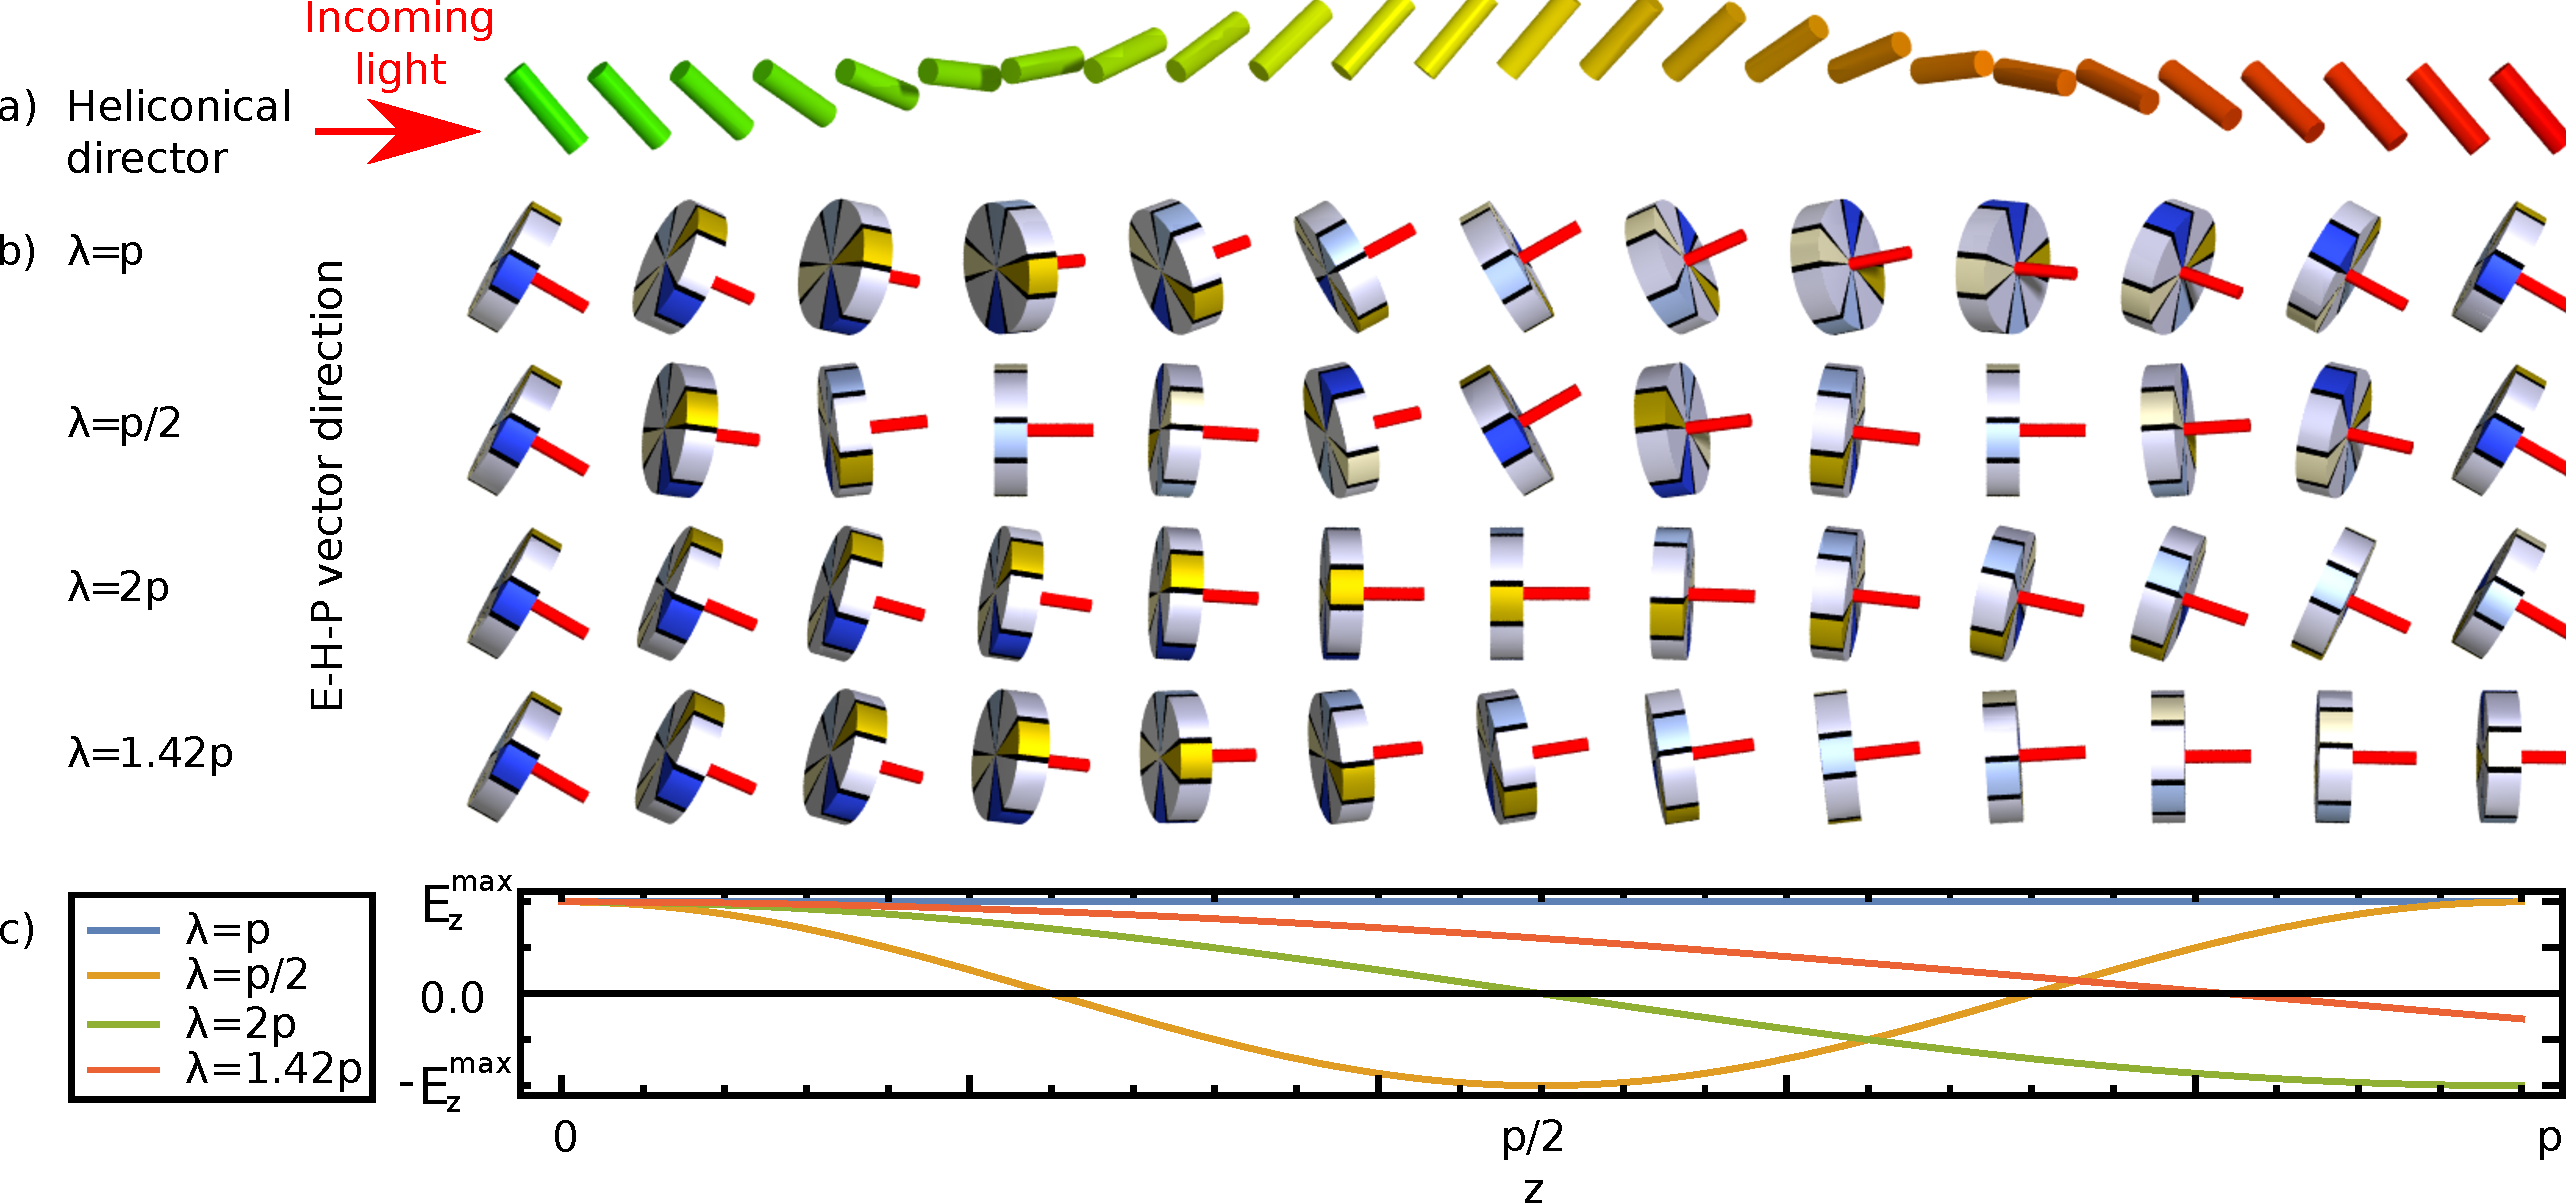
\includegraphics[height=140pt]{./figures/poynting-propagation1}}
    %\put(30,20){\includegraphics<2>[height=120pt]{./figures/poynting-propagation2}}
  \end{picture}}
  
  \vspace{-4.4cm}
  \item<2> On BG edge in one pitch length: $\vec{P}$ of RCP rotating circularly, $\vec{P}$ of LCP describing a four-leaf clover

% %     \put(0,30){\includegraphics<2->[height=80pt]{./slike/fig_frank_components_splay_s}}
%   \put(0,30){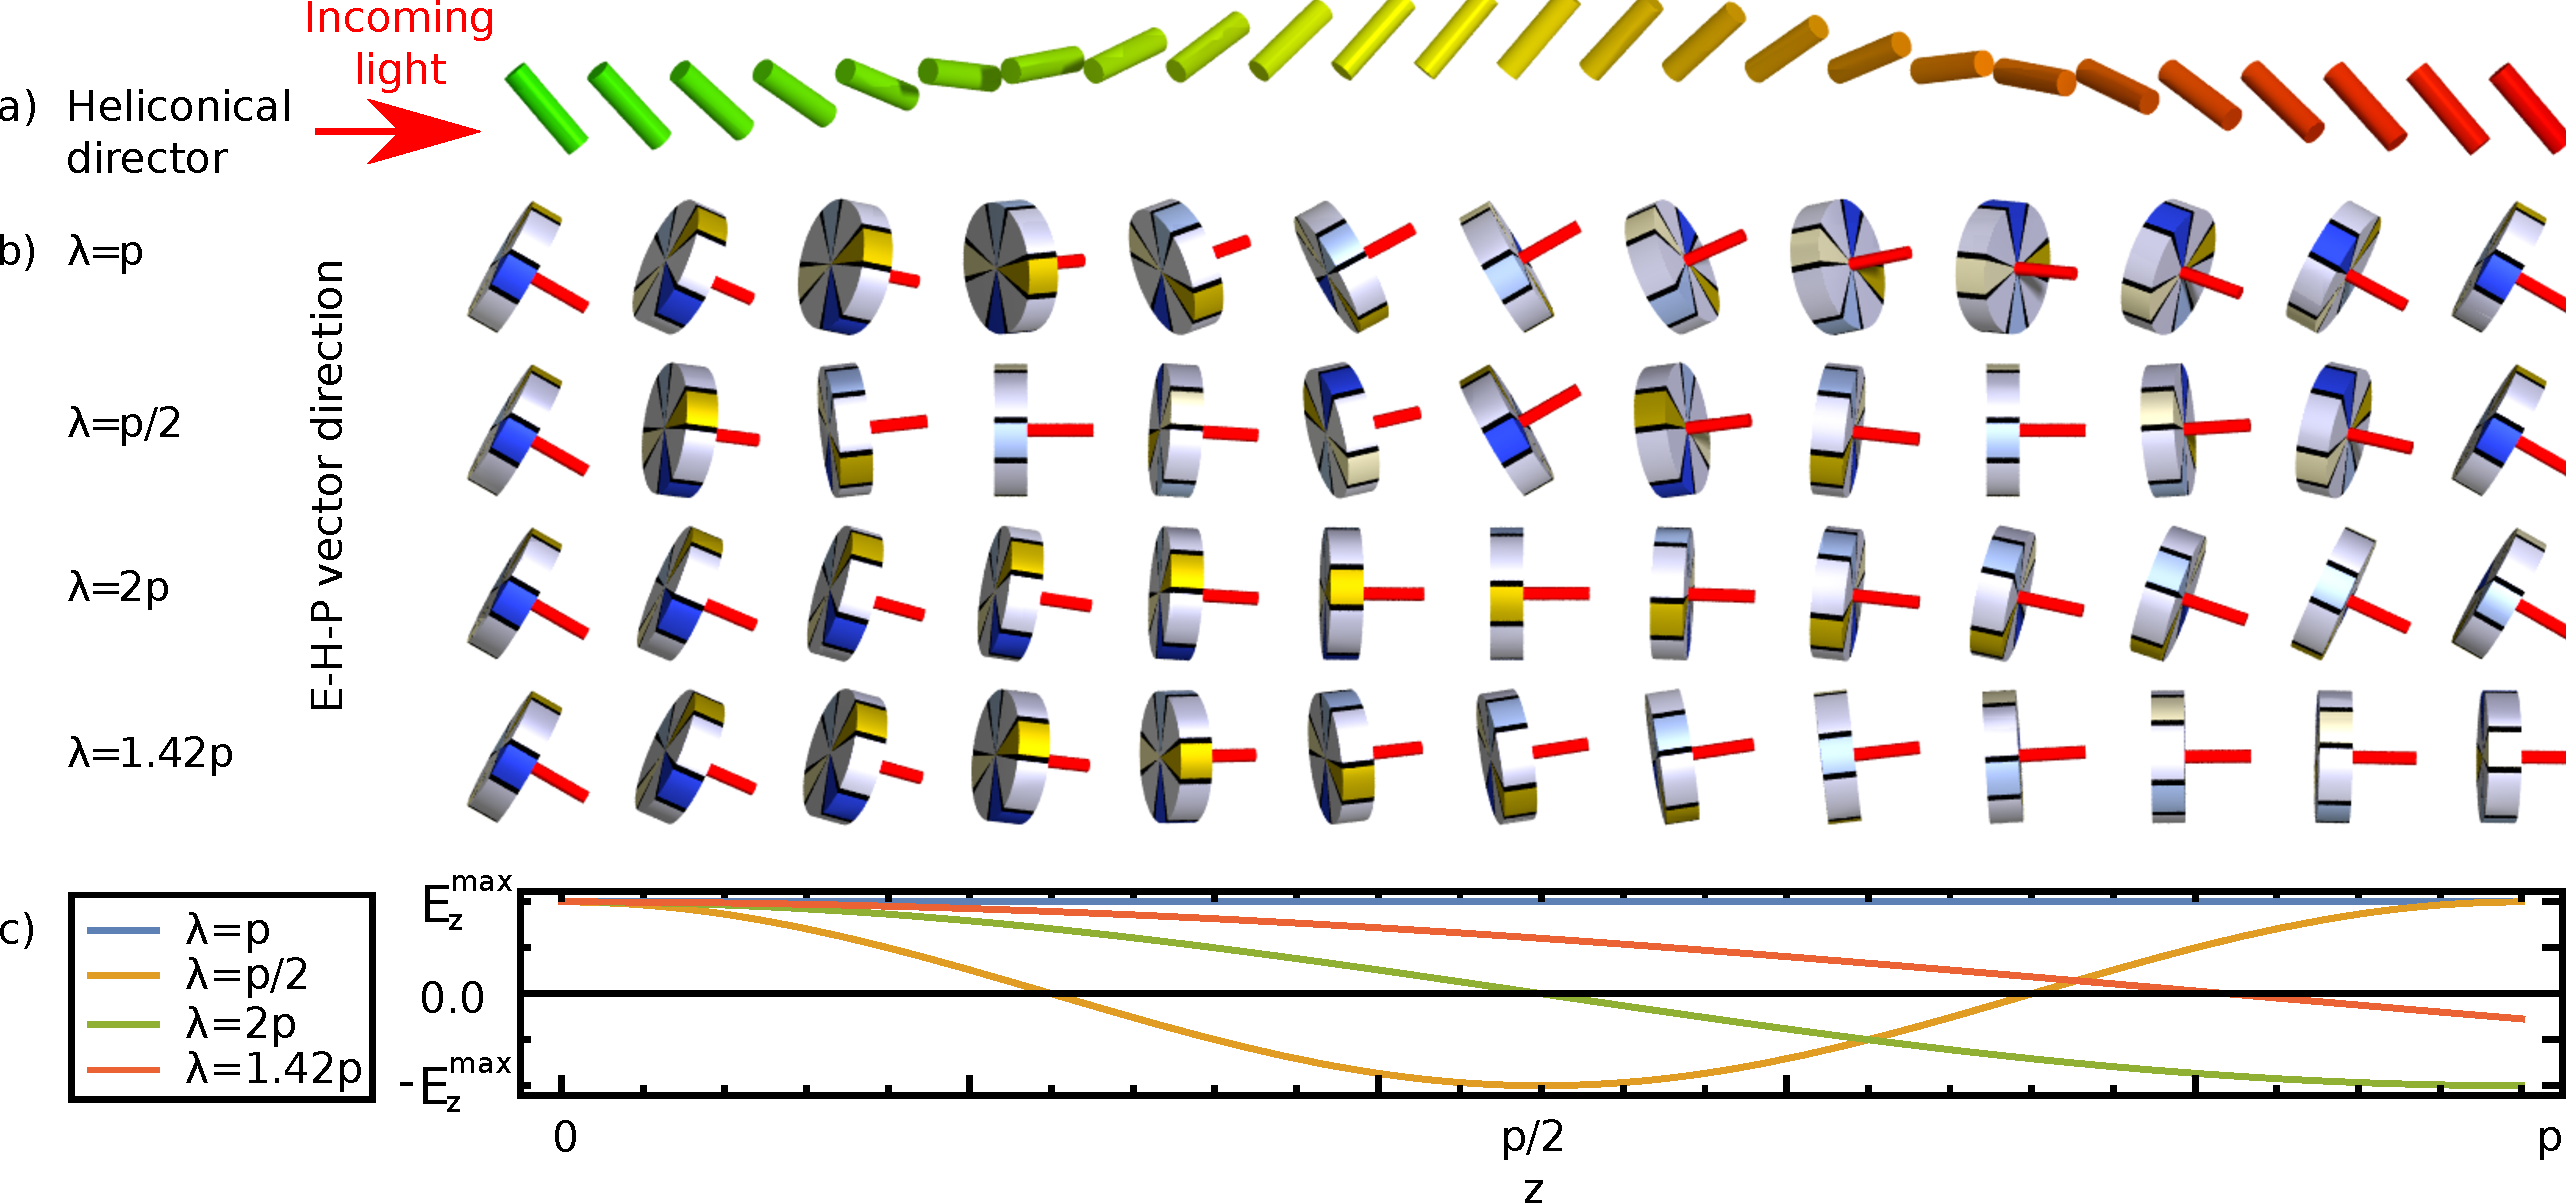
\includegraphics[height=150pt]{./figures/poynting-propagation1}}

\resizebox{\textwidth}{!}{\begin{picture}(400, 120)
  %\put(25,-30){\includegraphics<1>[height=140pt]{./figures/poynting-propagation1}}
  \put(-10,-20){\includegraphics<2>[height=120pt]{./figures/poynting-propagation2}}
\end{picture}}
%   \begin{overpic}[height=150pt]{./figures/Poynting-rotation}
%   \end{overpic}
\end{itemize}
\end{slide}


%   \resizebox{\textwidth}{!}{\begin{picture}(400, 120)
%     \put(0,30){\includegraphics<2->[height=80pt]{./slike/fig_frank_components_splay_s}}
%     \put(150,20){\includegraphics<2->[height=100pt]{./slike/fig_frank_components_twist_s}}
%     \put(270,30){\includegraphics<2->[height=80pt]{./slike/fig_frank_components_bend_s}}
%     \put(50, 10){\only<2->{\LARGE $\nabla \cdot \vec n$}}
%     \put(170, 10){\only<2->{\LARGE $\vec n \cdot \nabla \times \vec n$}}
%     \put(300, 10){\only<2->{\LARGE $\vec n \times \nabla \times \vec n$}}
%     \put(20, -20){\only<2->{\small P. G. de Gennes and J. Prost, The Physics of Liquid Crystals, Clarendon Press, 1993}}
%   \end{picture}}


\section{Conclusion}

\begin{slide}{Conclusion \& Outlook}
We determined the photonic properties of heliconical liquid crystals: 
\begin{itemize}
  \item The opening of the photonic band gap
  \item Analysis of $\vec{E}$ eigenmodes, the introduction of $E_z$ component
\end{itemize}
\end{slide}


% \begin{slide}{}
% \centering
%   \begin{overpic}[height=211pt]{./figures/ljubljana}
%   \put(40,52){Thank you!}
%   \end{overpic}
% \end{slide}



\end{document}








% SLAJD S POSTOPNIM PRIKAZOVANJEM BULLETOV: 
%
% \begin{slide}{Liquid crystals}
%  \begin{columns}[c]
%   \begin{column}{.5\textwidth}
%   
%    \begin{itemize}
%     \item Orientational order
%     \item Partional positional order\\[1em]
%     \item<2-> Control with external fields
%     %\item<2-> Elastic deformations of director
%     \item<2-> Birefringence
%    \end{itemize}
%   \end{column}
% 
%   \begin{column}{.5\textwidth}
%     \includegraphics[width=\textwidth]{./slike/faze_brez_crk}
%   \end{column}
%     
%   \end{columns}
% 
%   \resizebox{\textwidth}{!}{\begin{picture}(400, 120)
%     \put(0,30){\includegraphics<2->[height=80pt]{./slike/fig_frank_components_splay_s}}
%     \put(150,20){\includegraphics<2->[height=100pt]{./slike/fig_frank_components_twist_s}}
%     \put(270,30){\includegraphics<2->[height=80pt]{./slike/fig_frank_components_bend_s}}
%     \put(50, 10){\only<2->{\LARGE $\nabla \cdot \vec n$}}
%     \put(170, 10){\only<2->{\LARGE $\vec n \cdot \nabla \times \vec n$}}
%     \put(300, 10){\only<2->{\LARGE $\vec n \times \nabla \times \vec n$}}
%     \put(20, -20){\only<2->{\small P. G. de Gennes and J. Prost, The Physics of Liquid Crystals, Clarendon Press, 1993}}
%   \end{picture}}
%   
%   
% \end{slide}




% SLAJD Z UPORABO LEPIH KVADRATKOV Z NASLOVOM (\BEGIN{BLOCK}{NASLOV BLOKA})
% 
% \begin{slide}{Electromagnetic radiation}
% \vspace{-0.5cm}
% \begin{columns}[t]
% 
% \column{.6\textwidth}
%  
% \begin{block}{Maxwell's equations}
% \vspace{-0.5cm}
% \begin{equation*}
% \begin{aligned}
%  \nabla \cdot \vec D = \rho_f & \qquad \nabla \cdot \vec B = 0 \\
%  \nabla \times \vec E = -\odvod{\vec B}{t} & \qquad \nabla \times \vec H = \vec J_f + \odvod{\vec D}{t}
% \end{aligned} 
% \end{equation*}
% \end{block}
% 
%  \begin{block}{Describing metal and dielectrics}
% \begin{itemize}
%  \item Dissipative losses included with Lorentz/Drude model: $\eps(\omega)=1+\dfrac{\omega_p^2}{(\omega_0^2-\omega^2)-\mathrm{i}\Gamma\omega}$
%  \item $\mu$ presumed constant
% \end{itemize}
% \end{block}
% 
% % \only<1-1>{\vspace{9.75pt}}
% 
% \column{.35\textwidth}
% 
% \begin{block}{Constitutive relations}
% \vspace{-0.5cm}
% \begin{align*}
% \vec D &= \eps \varepsilon_0 \vec E \\ 
% \vec B &= \mu \mu_0 \vec H
% \end{align*}
% \end{block}
% 
% \begin{center}
%  \includegraphics[width=.9\textwidth]{./slike/metal-abs}
% \end{center}
% 
% \end{columns}
% \end{slide}






% SLAJD Z UPORABLJENO DRUGACNO BARVO BLOCKA (ZELENKASTA, UKAZ \BEGIN{EXAMPLEBLOCK})
% 
% \begin{slide}{Future work 1: Liquid crystal metamaterial -- shape}
% \vspace{-0.1cm}
% \begin{columns}
%   \column{.55\textwidth}
%   {\small \begin{block}{Shape research}
%    \begin{itemize}
%     \item Changing the optical axis of metamaterial in space and in time
%     \item Designing structures of liquid crystal metamaterial
%     \item Generalisation of 2D shapes to 3D
%     \item Generalisation to properties of homogeneous materials
%    \end{itemize} 
%   \end{block} }
%   
%   
%   
% %   \vspace{0.5cm}
% %   \includegraphics[width=.9\textwidth]{./slike/soukoulis1}
%   
% 
% 
%   
%   \column{.4\textwidth}
% 
%   \begin{center}
%   \includegraphics[width=.4\textwidth]{./slike/snowflake-mtm}
%   \includegraphics[width=.45\textwidth]{./slike/3d-mtm}
% 
%   \vspace{0.3cm}
%   {\small \begin{exampleblock}{Goal}
%     To determine novel approaches to control the flow-of-light microscopically using designed liquid crystal mesophases of different particles
%   \end{exampleblock} }
%   
% 
%   
% %    \begin{overpic}[width=.8\textwidth]{./Slike/tine_defekt_4}
% %   \put(1,-6) {\tiny Porenta et al., Soft Matter (2012)}
% %   \end{overpic}
% 
%   
%   \end{center}
%   
% \end{columns}
%   \begin{center}
%   {\footnotesize Experimental collaborators: Igor Muševič (IJS)}
%   \end{center}
%   
% \end{slide}



% SLAJDI ZA DODATEK (APPENDIX) -- da ti jih številči ločeno

% \appendix
% \backupbegin
% 
% 
% \begin{slide}{Free energy approach to heliconics}
% \end{slide}
% 
% \begin{slide}{Analytical expressions for $\vec{E}$ inside heliconics}
% \end{slide}
% 
% \begin{slide}{Winding of $\vec{P}_{xy}$ for different $\lambda/p$}
% \end{slide}
% 
% 
% \backupend



